% ****** Start of file apssamp.tex ******
%
%   This file is part of the APS files in the REVTeX 4.1 distribution.
%   Version 4.1r of REVTeX, August 2010
%
%   Copyright (c) 2009, 2010 The American Physical Society.
%
%   See the REVTeX 4 README file for restrictions and more information.
%
% TeX'ing this file requires that you have AMS-LaTeX 2.0 installed
% as well as the rest of the prerequisites for REVTeX 4.1
%
% See the REVTeX 4 README file
% It also requires running BibTeX. The commands are as follows:
%
%  1)  latex apssamp.tex
%  2)  bibtex apssamp
%  3)  latex apssamp.tex
%  4)  latex apssamp.tex
%
\documentclass[%
 reprint,
%superscriptaddress,
%groupedaddress,
%unsortedaddress,
%runinaddress,
%frontmatterverbose,
%preprint,
%showpacs,preprintnumbers,
%nofootinbib,
%nobibnotes,
%bibnotes,
 amsmath,amssymb,
 aps,
%pra,
%prb,
%rmp,
%prstab,
%prstper,
%floatfix,
]{revtex4-1}

\usepackage{float}
\usepackage{graphicx}% Include figure files
\usepackage{dcolumn}% Align table columns on decimal point
\usepackage{bm}% bold math
\usepackage{hyperref}% add hypertext capabilities
%\usepackage[mathlines]{lineno}% Enable numbering of text and display math
%\linenumbers\relax % Commence numbering lines
% \usepackage[toc,page]{appendix}
% \addbibresource{sample.bib}


%\usepackage[showframe,%Uncomment any one of the following lines to test
%%scale=0.7, marginratio={1:1, 2:3}, ignoreall,% default settings
%%text={7in,10in},centering,
%%margin=1.5in,
%%total={6.5in,8.75in}, top=1.2in, left=0.9in, includefoot,
%%height=10in,a5paper,hmargin={3cm,0.8in},
%]{geometry}

\begin{document}

%\preprint{APS/123-QED}

\title{LASSO or $L_1$ regularization in linear models}% Force line breaks with \\
% \thanks{Project in Advanced Methods in Applied Statistics}%

\author{Magnus Berg Sletfjerding}
 % \altaffiliation[Also at ]{Physics Department, XYZ University.}%Lines break automatically or can be forced with \\

\affiliation{%
 Copenhagen University
}%

\date{\today}% It is always \today, today,
             %  but any date may be explicitly specified

\begin{abstract}
  Least Squares Estimation of linear models are often prone to overfitting in higher dimensions.
  The LASSO penalty seeks to ameliorate this issue by introducing a penalty equal to the sum of the absolute value of the coefficients times a constant.
  Because the coefficients' absolute values are added linearly, not in quadrature, some LASSO coefficients are likely to be 0.
  This phenomenon gives the analyst the combined benefits of Ridge Regression and subset selection.
  To illustrate, the LASSO penalty is also applied on logistic regression.
  The subsequent combination is applied first on a known dataset, the South African Heart Disease set, and following tested on data obtained from 2014-2018 grade statistics at Copenhagen University.
\end{abstract}

\maketitle

%\tableofcontents
\section{Introduction}

Linear models for modelling data are among the first ones we encounter.
Both from a mathematics perspective, where $y = ax + b$ is hammered into the heads of every high school freshman, but also in daily life, where we assume that if one person eats two apples, two must eat four.\cite{sterling_1001_2013} %find a HS textbook to cite
The simplicity of linear models are part of the reason they are so widely applied.
This is also true from a computational perspective; a linear regression or classification model is orders of magnitude faster to train than a neural network predictor, and can often outperform more complex models. \cite{hastie_elements_2017}

However, as the systems we analyze become more and more complex, and as our datasets increase in dimensionality, classical linear models become too complex. \cite{efron_least_2004}
Although somewhat outdated \cite{courtney_comments_2008}, Occam's razor still applies - a simpler model can both be more accurate, and easier to interpret, than a complex one.
There are two common ways to simplify linear models.
The first is called subset selection - and relies on either removing or adding one parameter at a time, to find the variables that are "most important" in a model.
I will not discuss subset selection at length in this report.
The second way to simplify a linear model is called shrinkage, and involves adding a penalty on the size of the fit parameters when fitting the linear model to data.
The LASSO, or the least absolute shrinkage and selection operator, though formally a shrinkage method, also functions as a subset selector.
By pushing vector values towards 0, the LASSO allows for fitting sparse, multidimensional data to a linear model, which does not need to take all features of the data into account.

The LASSO penalty is not limited to linear regression, however.
In fact, logistic regression can also use the LASSO penalty to overcome overfitting when classifying data in higher dimensions.
In this report, I will give a general introduction to the LASSO penalty in linear regression, and then show how it can be used in logistic regression for binary classification.

Finally, I show how logistic regression can be used to identify the grades from Copenhagen University's SCIENCE faculty compared to all other faculties, with a 68.5\% accuracy.


\section{The LASSO}

\subsection{General problem}
If we consider a regression problem $y = Xw$, where X is our input, y is the output, and w is the weight vector for each dimension of X.
\[
y = [y_1, y_2, ..., y_i]^T
\]
\[
X = [x_1^T, x_2^T, ..., x_i^T]^T
\]
\[
x_i = [1,x_{i1},x_{i2},...,x_{ij}]^T
\]
\[
w = [w_0, w_1, ...  w_j]^T
\]
We include a 1 in the first dimension of $x_i$ to account for the intercept, $w_0$.
Alternately, we can write the problem like this:
\[
y_i \approx f(x_i;w) = w_0 + \sum_{j=1}^{d}x_{ij}\cdot w_j
\]
Or, in short form:
\[
y_i \approx f(x_i;w) = x_{i}^T\cdot w
\]
Where f is a function, mapping the inputs ($x_i$) to outputs ($y_i$)
The fastest way to find the optimum parameters of w (or, "fitting" f to the data), is to minimize the least squares (or $\chi^2$) objective, which is:
\[
\sum^n_{i=1}(y_i - f(x_i;w))^2 = \lvert\lvert y - Xw \rvert\rvert^2_2
\]
Here, $\lvert\lvert y - Xw \rvert\rvert_2$ refers to the $l_2$ norm of $y - Xw$, or:
\[
\lvert\lvert y - Xw \rvert\rvert_2 = (\sum_{j=1}^d (\lvert w_j \rvert^2) )^{\frac{1}{2}}
\]
And, if we assume the distribution of our variables is Gaussian, the least squares solution is equal to the maximum likelihood solution. \cite{paisley_columbiax:_2018}

However, the least squares objective is a bit difficult to work with once our data vector X starts reaching higher dimensions.
This is especially due to the added sparsity that comes with higher dimensionality, and the accuracy of our predictor will decrease if we overfit to the training data.
More often than not, we deal with features that have little or no importance to our results.
In this case, it becomes more interesting to have certain weights equal to zero, such that some variables have no contribution towards the predicted value:
\[
f(x_i;w) = w_0 * 1 + w_1 x_1 + ... + 0 * x_k + ... w_j x_ij
\]


\subsection{The LASSO objective}

The least absolute shrinkage and selection operator, or the LASSO, regularizes the least squares objective with a penalty on the size of w.
LASSO regression minimizes the following objective function:
\[
\lvert\lvert y - Xw \rvert\rvert^2_2 + \lambda \lvert\lvert w \rvert\rvert_1
\]
where we have our penalty function:
\[
\lvert\lvert w \rvert\rvert_1 = \sum^n_{i=1}\lvert w_i \rvert
\]
and $\lambda$ is a regularization parameter to be set by the user.
\cite{tibshirani_regression_1996}

A graphical illustration of the LASSO penalty is given in figure \ref{LASSOexplained}.

\begin{figure}
  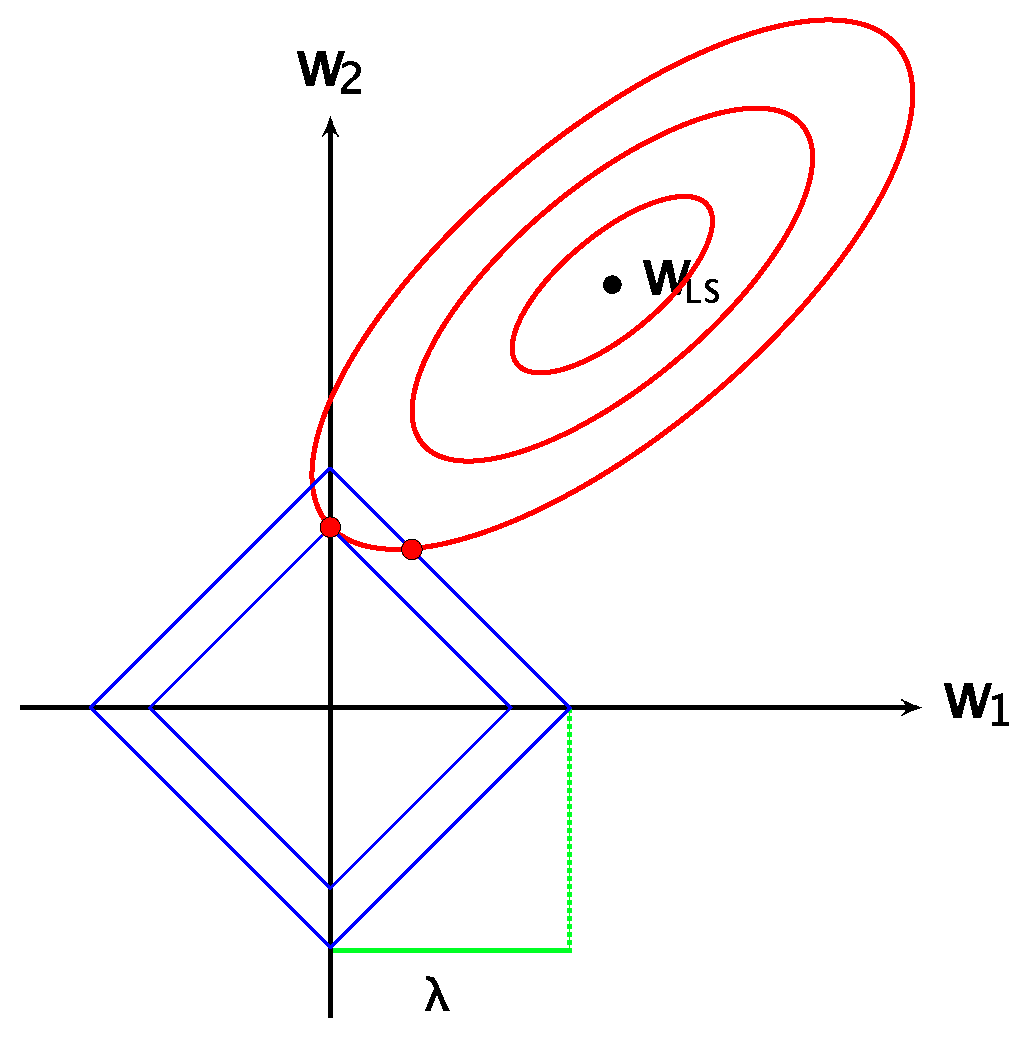
\includegraphics[width=\linewidth]{../figs/ill_LASSO}
  \caption{Illustration of the principle of LASSO.
  $w_{LS}$ is the least squares estimate of w.
  The red lines are the contours of $\lvert\lvert y - Xw \rvert\rvert_2^2$, similar to a likelihood contour.
  The blue lines are the contours of $\lvert\lvert w \rvert\rvert_1$, at two different values of $\lambda$ (one is labelled in green).
  Two red dots are plotted, showing vector solutions $w$ for each of the two $\lambda$ values.
  That is, they are minima of $\lvert\lvert y - Xw \rvert\rvert^2_2 + \lambda \lvert\lvert w \rvert\rvert_1$ for two different $\lambda$s.
  As can be seen, for the lower value of $\lambda$, $w_2 = 0$, as was part of the objective.
  }
  \label{LASSOexplained}
\end{figure}



\subsection{Consequences of using a LASSO penalty}
The advantage of using a LASSO penalty (compared to using none) on $w$ is evident when we plot the coefficients of $w$ as a function of $\lambda$, as in figure \ref{LASSOpath}, using the diabetes dataset of \texttt{sklearn}. \cite{pedregosa_scikit-learn:_2011}
Here, we see that a significant portion of the coefficients are zero at low values of $\lambda$, neatly following Occam's razor. \cite{tibshirani_regression_1996}


\begin{figure}
  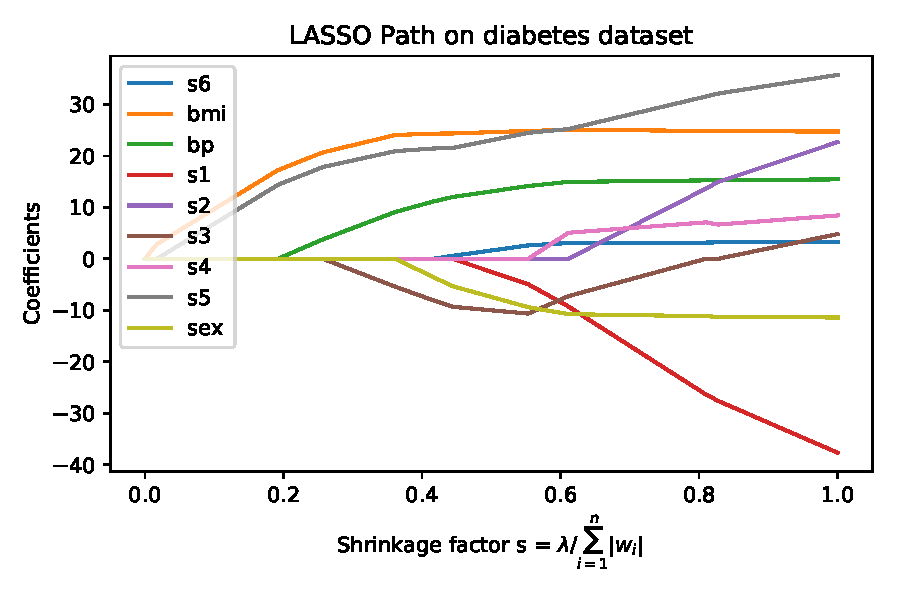
\includegraphics[width=\linewidth]{../figs/LASSO_paths}
  \caption{Profiles of LASSO coefficients as the tuning parameter is increased. Lines are drawn at the parameter value at which a new nonzero coefficient is included.
  As can be seen, two out of the three largest values at $\lambda = 1$ are already singled out before $\lambda = 0.1$.
  When the shrinkage factor s = 1, $w_{lasso} = w_{ls}$, the least squares estimate, while if s = 0, all coefficients are zero, as the penalty on $w$ is infinity.
  }
  \label{LASSOpath}
\end{figure}


\section{Logistic Regression}
Logistic regression is a linear classification method, which predicts the a binary class $y_i$ for each data point $x_i$.

\subsection{General form}
Assume sets of data points $(x_1, y_1), ... , (x_i, y_i)$ where $x_i$ is defined as before and $y_i \in \{-1, +1\}$.

We can predict the value of y using a linear function, using a weight vector as before:
\[
y_i = sign(x_{i}^T\cdot w)
\]
This is the general \textbf{linear classifier}, which follows a Bernoulli distribution.

The weight vector $w$ acts as a classifier based on a hyperplane, as described in figure \ref{hyperplane}.

\begin{figure}
  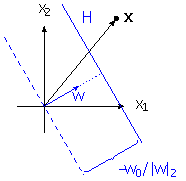
\includegraphics[width=\linewidth]{../figs/hyperplane}
  \caption{
  Illustration of the principle of a hyperplane in 2 dimensions (in this case, a hyper-line).
  x signifies a vector $x = [ 1, x_1, x_2 ]^T$, while $w = [ w_0, w_1, w_2 ]^T$.
  The hyperplane $H$ is perpendicular to $w$, and classifies $x$.
  As $x$ lies in the positive direction of $H$ (that is, the direction of $w$) $y=1$ for this particular x.
  The offset of the hyperplane ($w_0$) is also signified.
  }
  \label{hyperplane}
\end{figure}

\subsection{Logistic link (sigmoid) function}
While the separation based on the sign of $x_{i}^T\cdot w$ is useful, logistic regression expands upon this to include a probability as well.

To find the probability of a data point belonging to a certain class, we set the log odds equal to the linear classifier core function:

\[
ln \frac{p(y = +1|x)}{p(y = +1|x)} = x_{i}^T\cdot w
\]
Where $p(y = +1|x) = 1 - p(y = +1|x)$, naturally.

This allows us to solve for $p(y = +1|x)$:
\[
p(y = +1|x) = \frac{e^{x_{i}^T\cdot w}}{1 + e^{x_{i}^T\cdot w}} = \sigma(x_{i}^T\cdot w)
\]
This is known as a \textit{sigmoid function} and is illustrated in figure \ref{sigmoid}.
\begin{figure}
  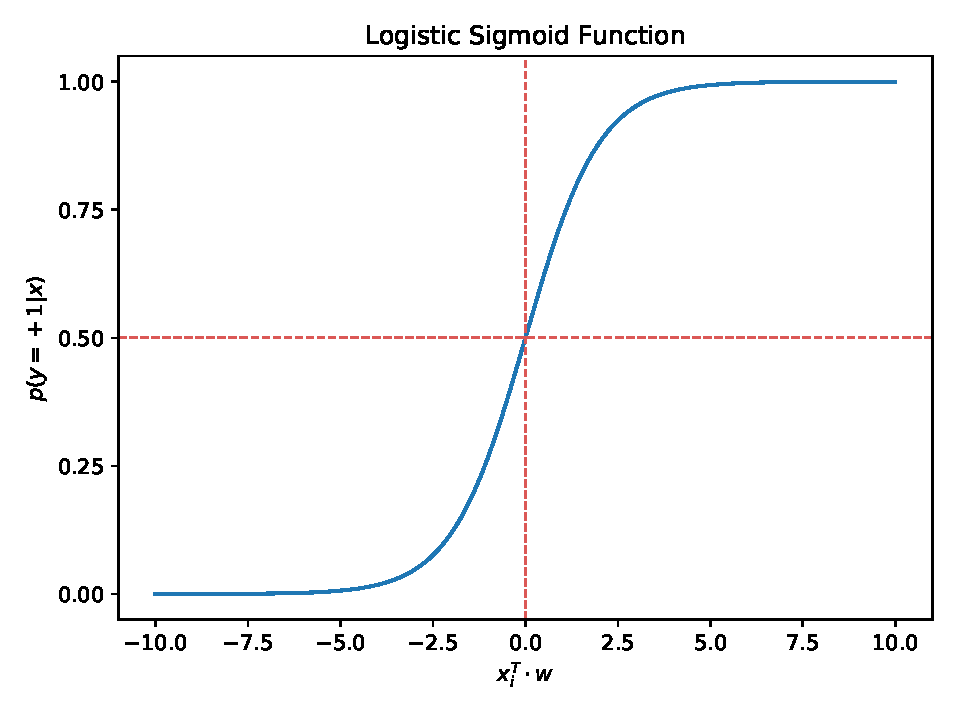
\includegraphics[width=\linewidth]{../figs/sigmoid}
  \caption{Sigmoid function of link function ($x_{i}^T\cdot w$).
  As the link function moves further away from 0, the probability increases or decreases accordingly.
  }
  \label{sigmoid}
\end{figure}

From the figure, we can see the following:
\[x_{i}^T\cdot w \to \infty, p(y = +1|x) \to 1\]
\[x_{i}^T\cdot w \to -\infty, p(y = +1|x) \to 0\]
\[x_{i}^T\cdot w = 0 \Leftrightarrow p(y = +1|x) = 0.5\]. % CONSIDER MAKING A TABLE


Essentially, the more positive the value of $x_{i}^T\cdot w$ is, the more confident we are that it belongs to class $y_i = +1$, and vice versa.


\subsubsection{Finding the optimum value of w}
In order to find the value of w which separates all training data, we find the value of $w$ which maximizes the log likelihood:
\[
ln(\mathcal{L}) = \sum_{i=1}^{n}ln \frac{e^{y_ix_i^Tw}}{1 + e^{y_ix_i^Tw}} = \sum_{i=1}^{n}ln \sigma(y_i\cdot w)
\]


\subsection{Regularization}
As before, Occam's razor applies; the simpler the model, the better.
Given that if the data is perfectly separable by a given hyperplane, we want to minimize the coefficients of $w$.

We therefore put a LASSO or $L_1$ penalty on the model, to get the $L_1$ regularized Logistic Regression objective:

\[
\sum_{i=1}^{n}ln \sigma(y_i\cdot w) - \lambda \sum_{j=1}^d \lvert w_j\rvert
\]
Note here that we subtract the penalty rather than add it, as the logistic regression is a maximization problem.


\subsection{$L_1$ regularized Logistic Regression on South African Heart Disease dataset}

I found the regularized Logistic regression implemented in \verb!sklearn.linear_model!, with an l1 penalty.
I used the dataset on South African heart disease\cite{hastie_elements_2017} to test it, and plotted the results in figure \ref{SAHeart}

 \begin{figure}
   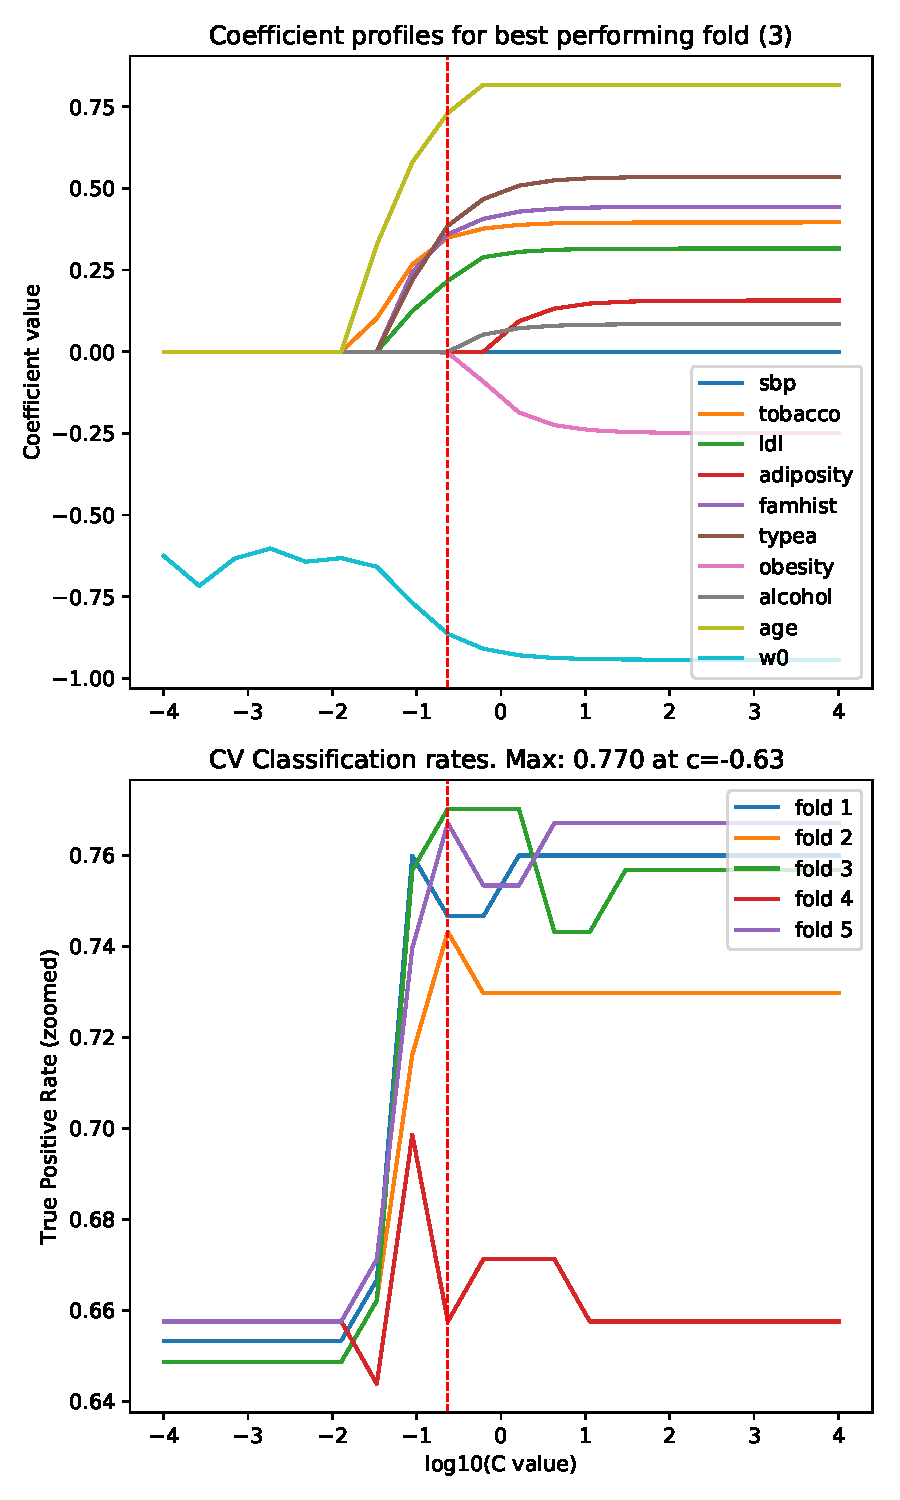
\includegraphics[width=\linewidth]{../figs/LogRegCV}
   \caption{L1 Regularized Logistic Regression on South African Heart Disease data
   \textbf{Top}: Coefficient paths, as in figure \ref{LASSOpath}, for the best performing cross validation fold.
   I used 5 random folds in total.
   \textbf{Bottom}: Classification rates for the 5 folds. Interestingly, the maximum rate of classification occurs while the coefficients for alcohol use, obesity, and adiposity are still zero, suggesting that these variables are sensistive to overfitting.
   }
   \label{SAHeart}
 \end{figure}


\section{Copenhagen University grade statistics}
Once I made sure that the Logistic Regression worked, I was lured in by the grade statistics of Copenhagen university.\cite{noauthor_karakterfordeling_nodate}
After a short discussion with some of my colleagues, we all agreed that courses at SCIENCE were significantly more challenging than at the HUM or SAMF faculty.
With this newfound (and slightly biased) hypothesis, I set out to see if there were grounds for this hypothesis, based on the grade statistics available online.

\subsection{Scraping and retrieving data}
I used the \texttt{selenium} package with the Chrome webdriver to extract the links to all courses and all semesters available, going all the way back to 2014. \cite{noauthor_selenium_nodate}
I then used \texttt{scrapy} to extract the necessary data from each page, and subsequently cleaned and formatted the data using the \texttt{pandas} library. \cite{noauthor_scrapy_nodate}\cite{mckinney_data_2010}
\subsection{Data cleaning and removal}
The first look at the data showed the following,
\begin{verbatim}
  fac
HUM        12842
JUR         1403
SAMF        4411
SCIENCE     7656
SUND        3246
TEO          699
\end{verbatim}
I decided only to work with courses that used the 7 point scale, as the pass/fail scale in reality only provides two dimensions - the number of students and the percentage of passing students.
\begin{verbatim}
  fac
HUM        5274
JUR         981
SAMF       2379
SCIENCE    4961
SUND       1871
TEO         296
\end{verbatim}
I then decided to include TEO in HUM and JUR in SAMF, as the content is both similar, and for the simple fact the statistics for those are significantly lower.
So I ended up with this:
\begin{verbatim}
  fac
HUM        5570
SAMF       3360
SCIENCE    4961
SUND       1871
\end{verbatim}

\subsection{Initial view of the data}
\begin{figure}[H]
  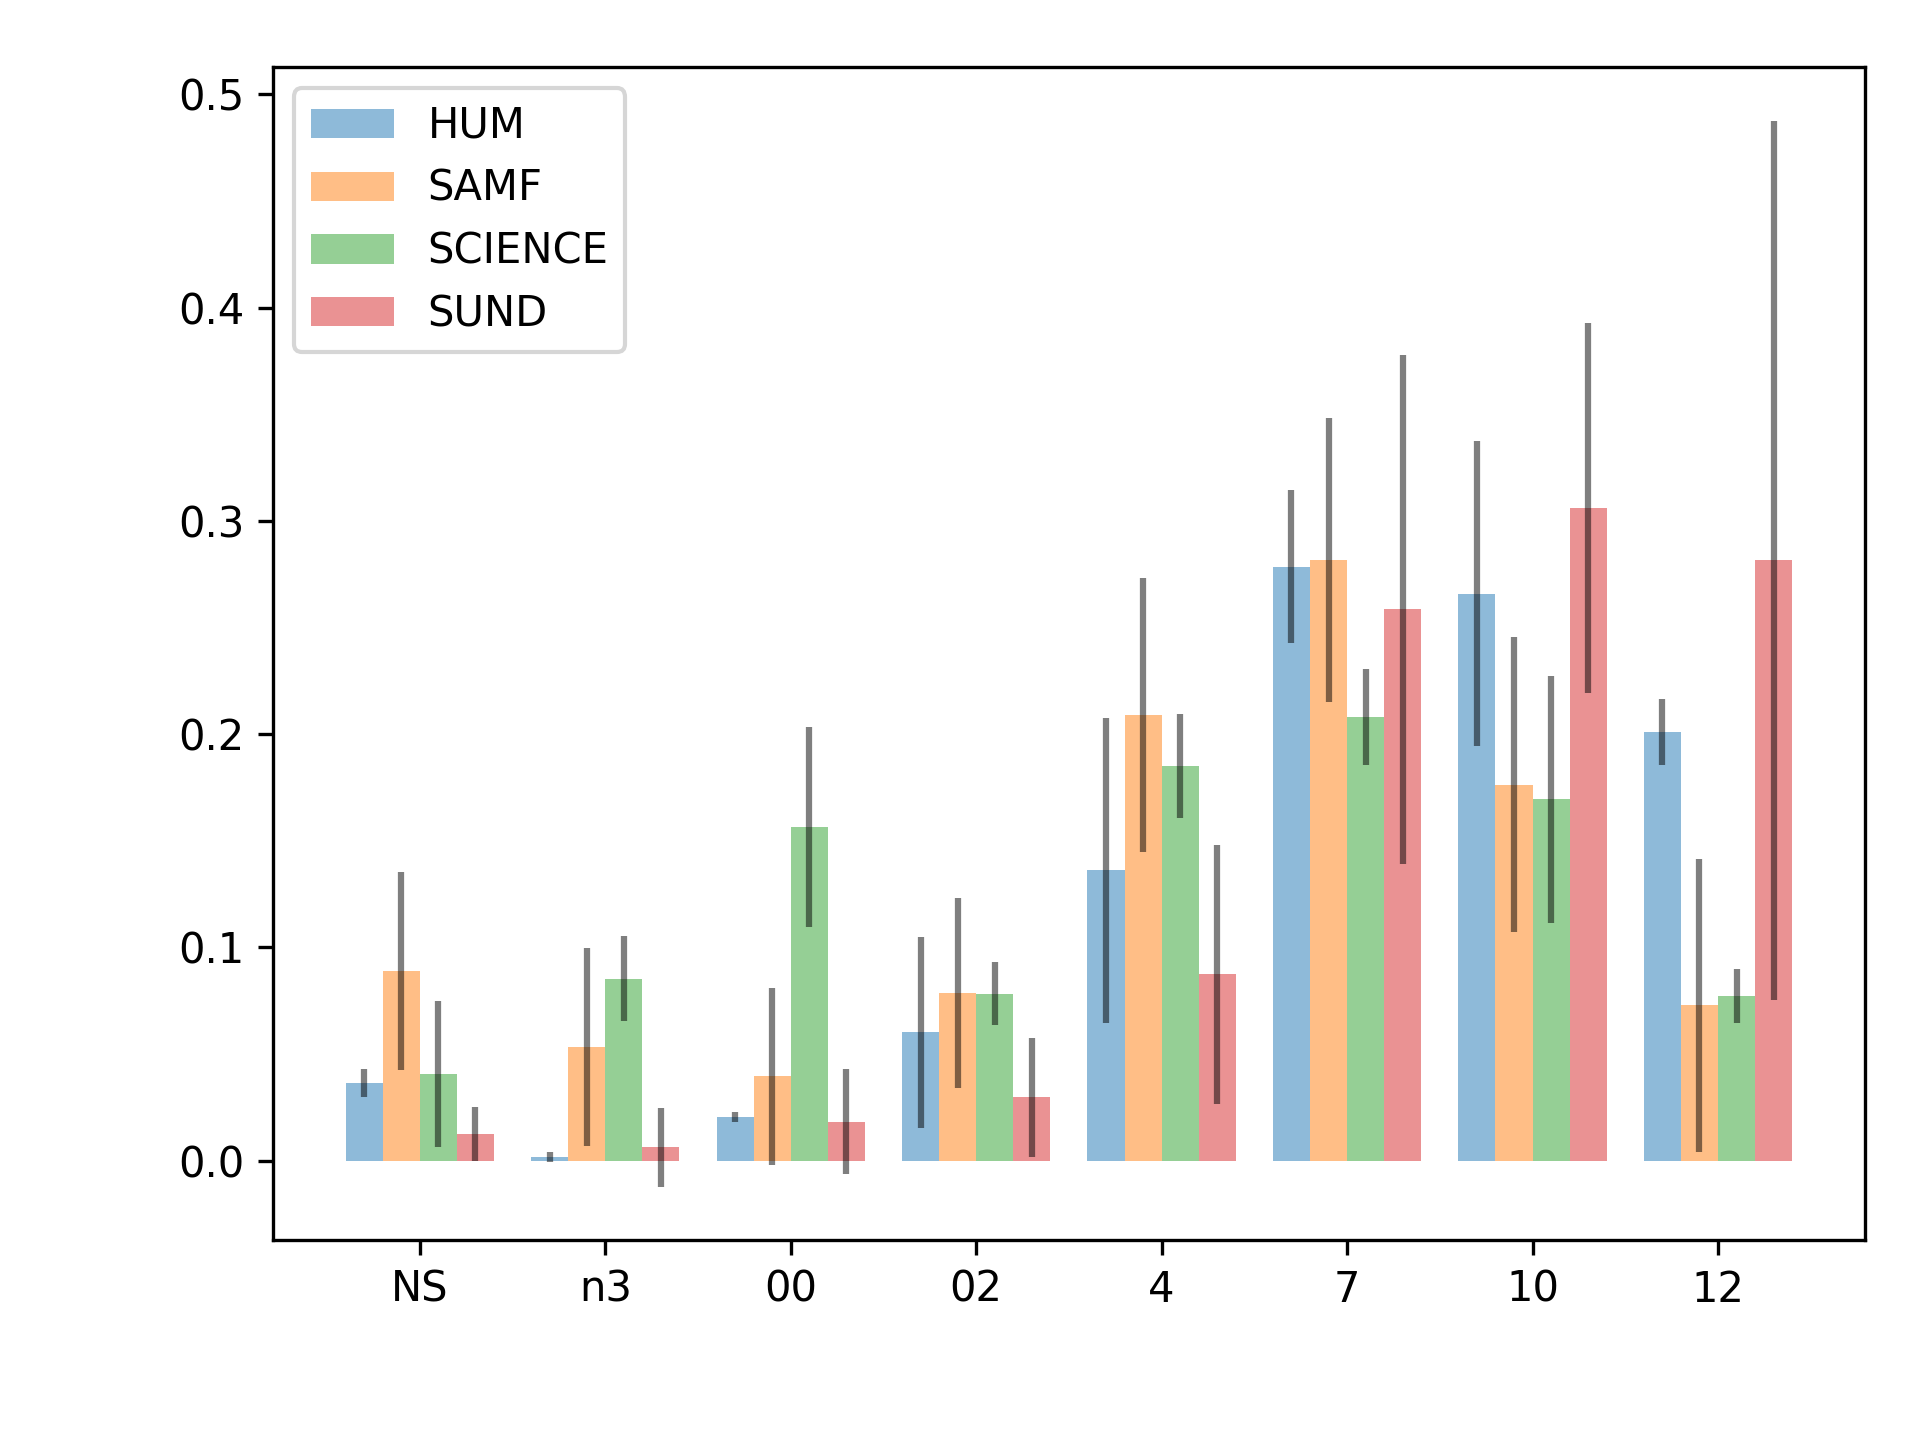
\includegraphics[width=\linewidth]{../figs/overlay.png}
  \caption{Bar plots of the four distributions of grades.
  Values are calculated as the mean ratio of each grade, with the error as the standard deviation on the mean.
  NS means "No show".
  As is evident, SCIENCE does differ slightly from the other faculties, with signifcantly more 00 grades.}
  \label{overlayKU}
\end{figure}
I noticed from figure \ref{overlayKU} that SCIENCE had a larger portion 00 grades when compared to the other faculties.
This could indicate that the courses indeed are harder, as the error bars do not overlap.


\subsection{Classifying SCIENCE vs not-SCIENCE}
Finally, I investigated the most pressing question of all: "Is SCIENCE all that special?" or, in other words, "At what rate is it possible to differentiate SCIENCE from other faculties based on the grades to their respective courses?"
I used the method already discussed (Logistic Regression with an l1 penalty) to try to differentiate between SCIENCE and "not SCIENCE," as Logistic regression is a binary classifier, and the fact that SCIENCE has the grade distribution (see figure \ref{overlayKU}) that differs the most from the other ones.

\begin{figure}
  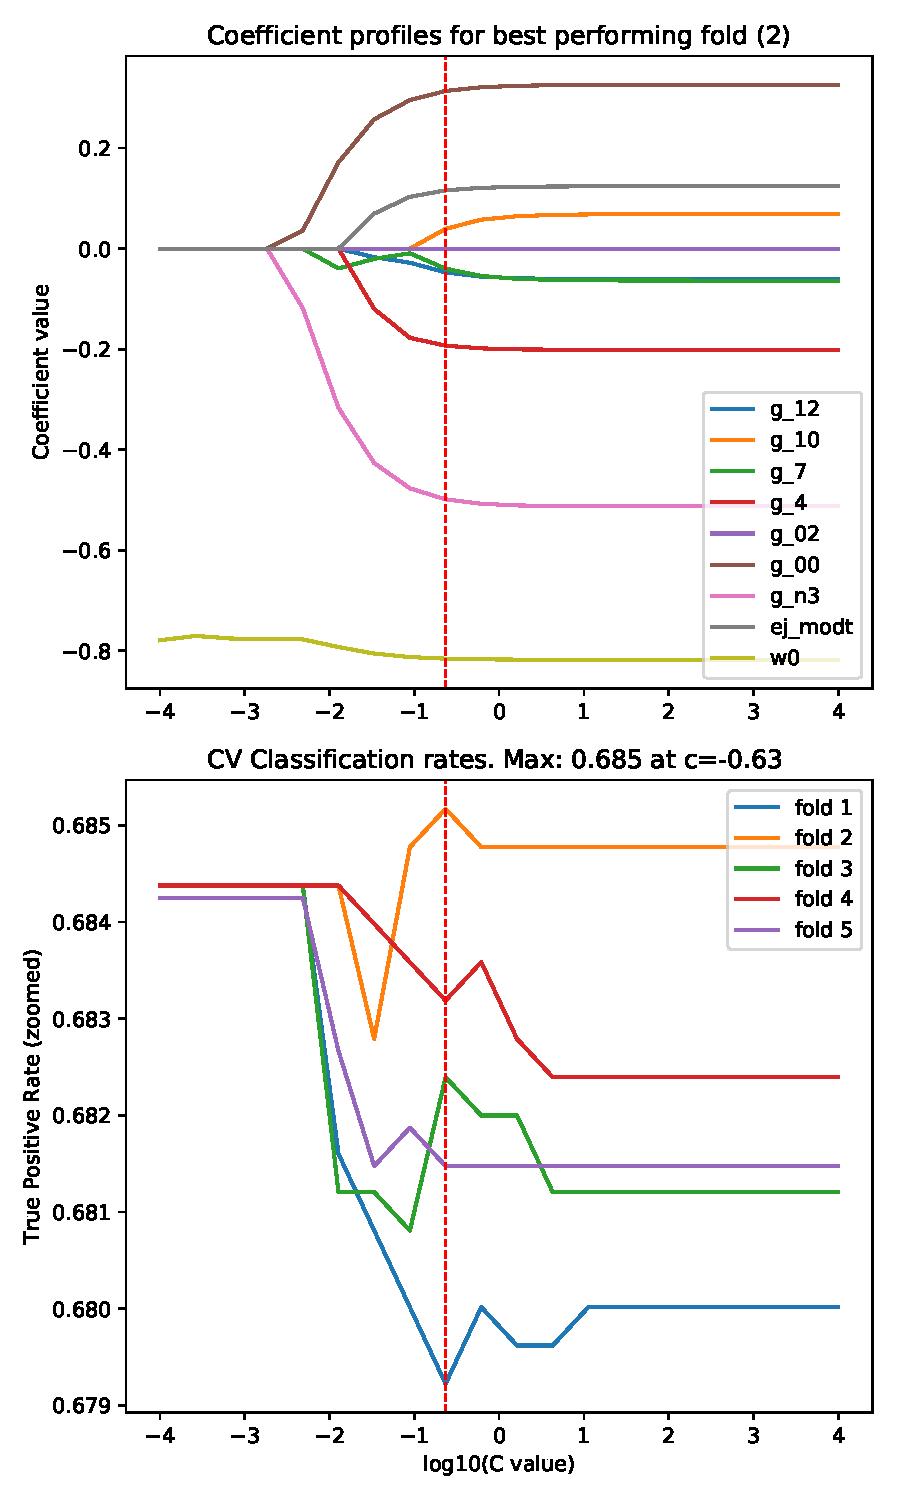
\includegraphics[width=0.9\linewidth]{../figs/LogRegCV_KU.pdf}
  \caption{L1 Regularized Logistic Regression on KU grade data
  \textbf{Top}: Coefficient paths, as in figure \ref{LASSOpath}, for the best performing cross validation fold.
  I used 5 random folds in total.
  \textbf{Bottom}: Classification rates for the 5 folds. The 2nd fold seems to outperform the others, for some reason.
  Again we see that some constraint on the weight vector yields a better classification rate.
  Interestingly, I did not get significantly higher rates of classification after either filtering the data by the nubmer of students, or by feature engineering more variables, as can be seen in the Appendix.
  }
  \label{}
\end{figure}


\section{Concluding remarks}
The properties of the LASSO are astonishing indeed.
One of the reasons why it is useful to work with is its simplicity - the sub of absolute values of coefficients is astonishingly easy to relate to.
Furthermore, the models that it can produce are insanely useful tools for understanding data in higher dimension.
When coupled with feature engineering and further selection, the LASSO penalty will also have the potential to find quadratic and other similar trends in data.

More often than not, students of statistics courses are absorbed into Machine Learning algorithms.
The elegance and purity of this method illustrate how important simple models are still relevant for statistical treatment of data.
\newpage
\bibliography{adv_app_stat}
\bibliographystyle{abbrvnat}

\end{document}
%
% ****** End of file apssamp.tex ******
